\problem{Quadratic Values}

\begin{enumerate}
    \item Plot the equation $y = x^2 - 1$ for $-5 < x < 5$
    \item What is the minimum?
\end{enumerate}

\solution

\part 

Using the following python code:

\inputminted{python}{code/p1.py}

\begin{center}
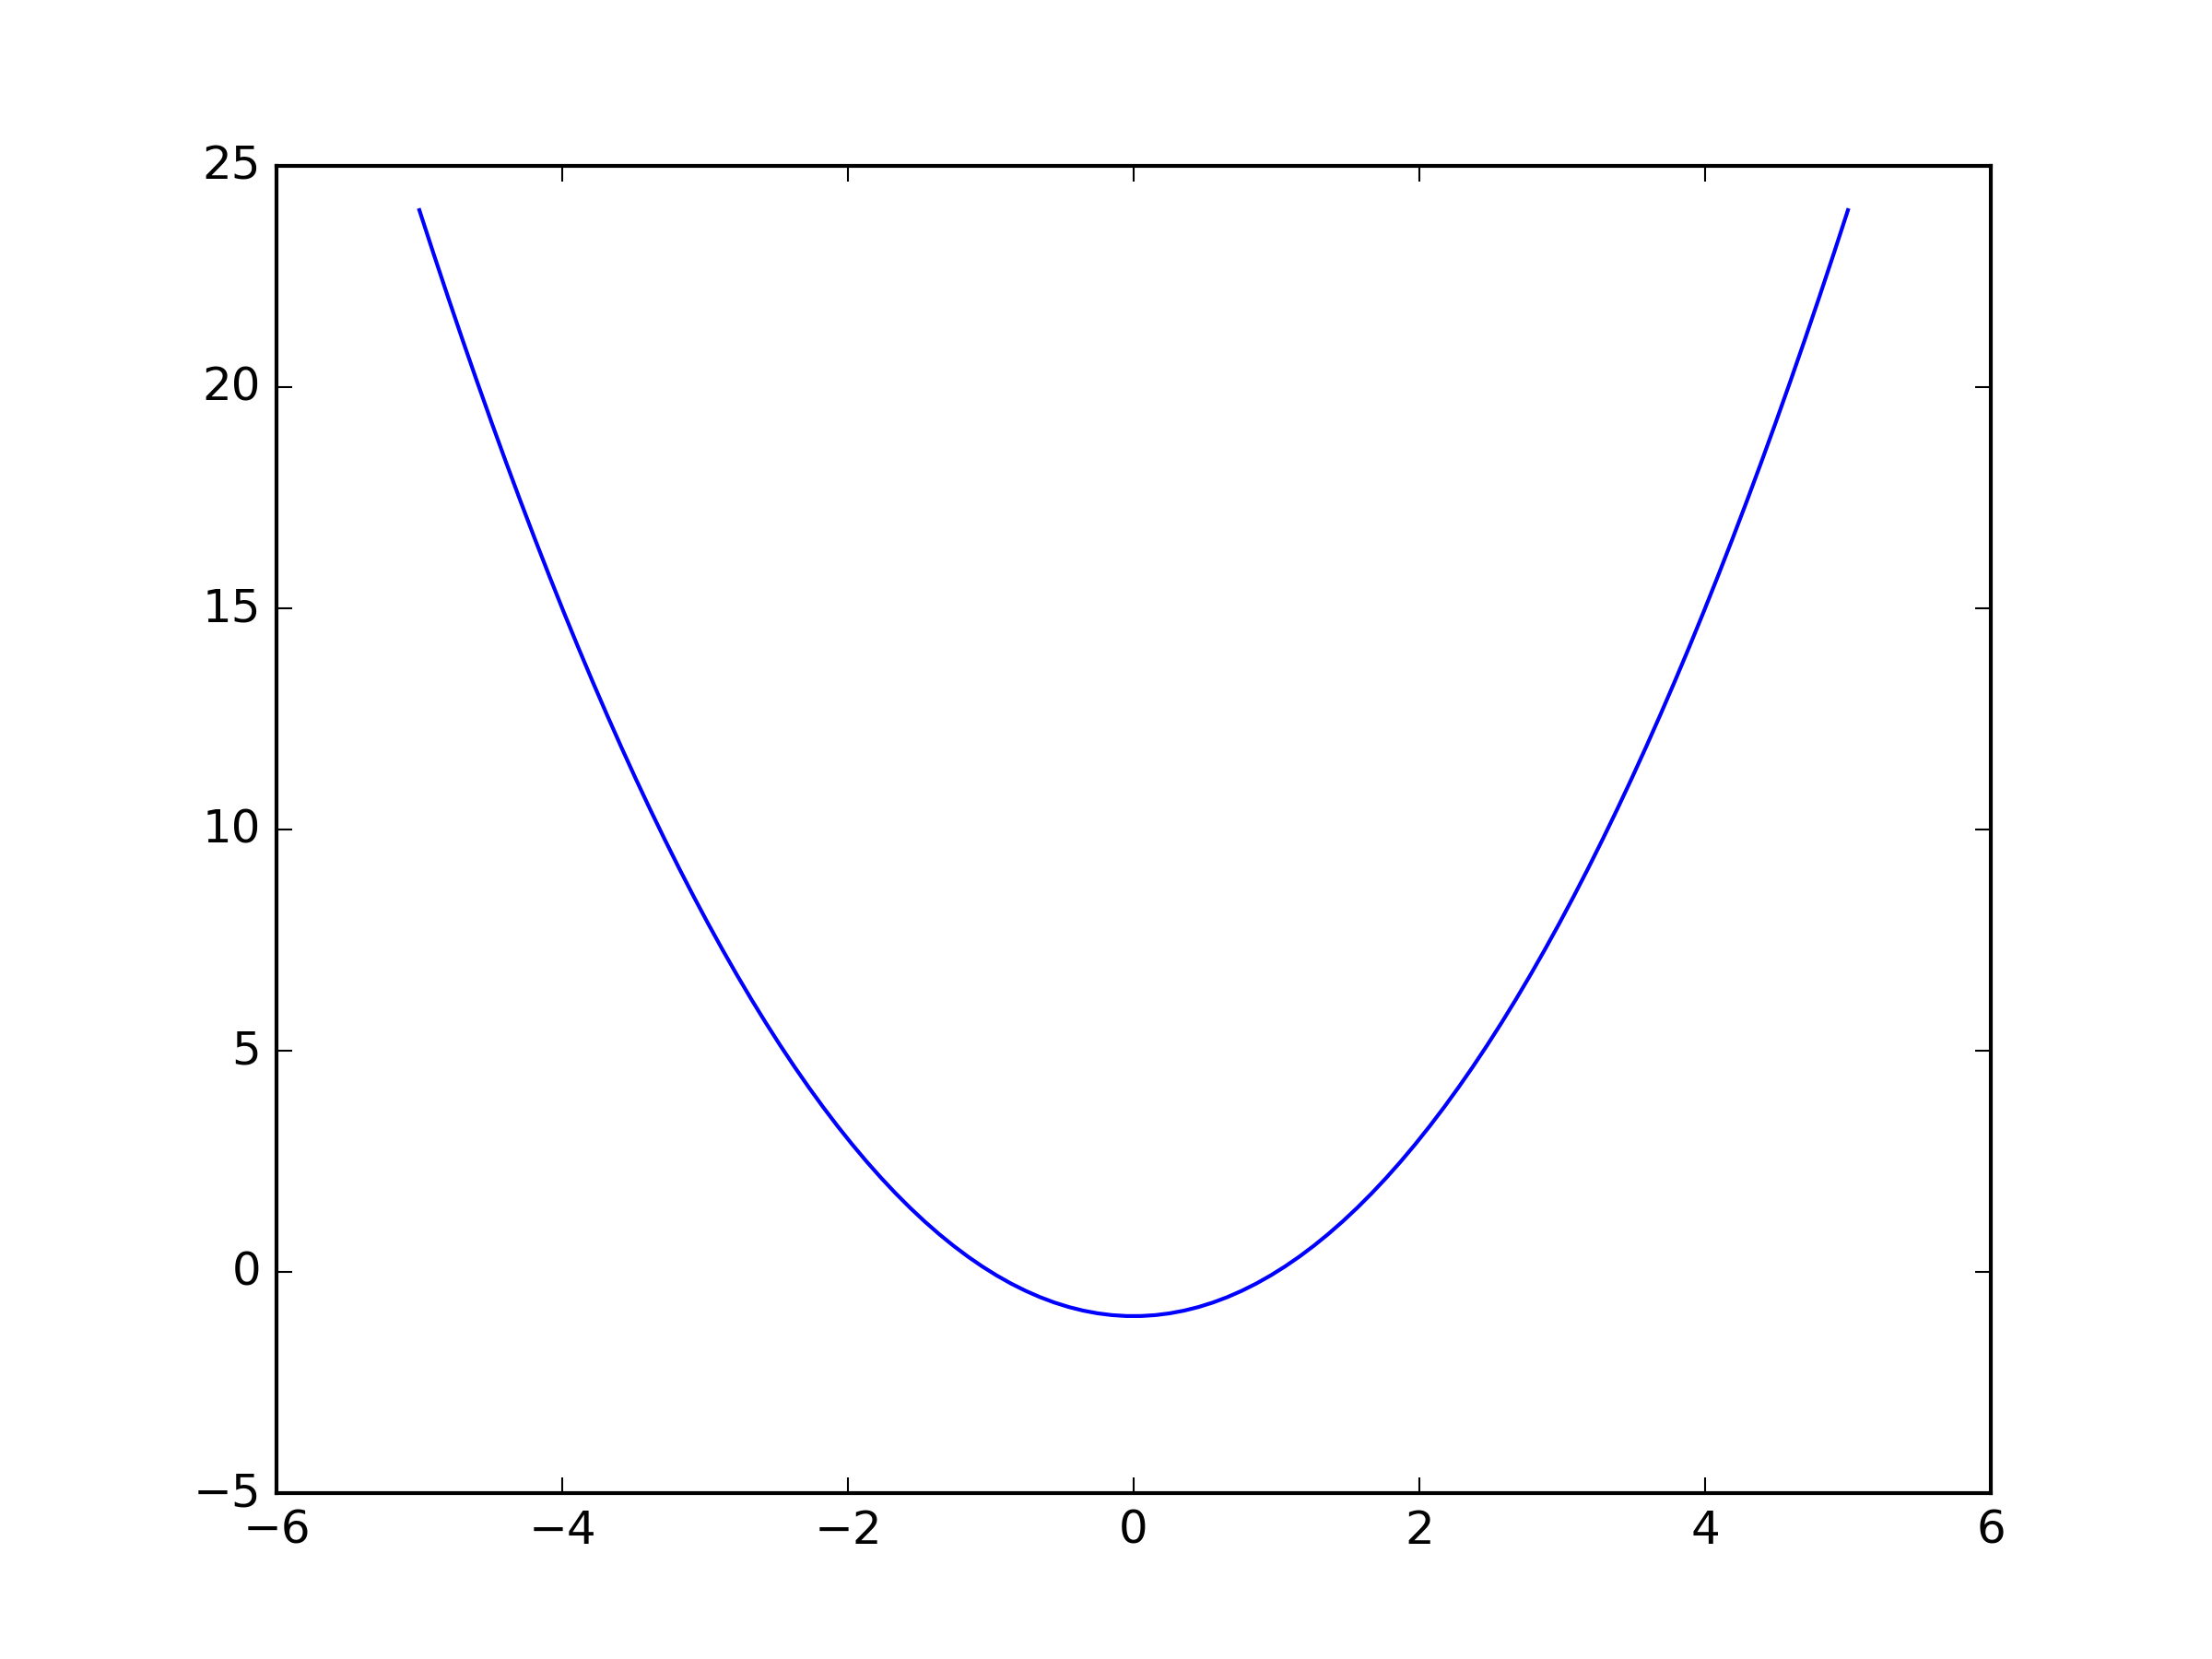
\includegraphics[width=.5\textwidth]{images/p1.png}
\end{center}

\part

The minimum is found by looking for zeros in the derivative.

$$ \frac{\partial y}{\partial x} = 2x$$

This has a zero at \fbox{$x = 0$}.